% ============================================================
%  AAAI 2027 Anonymous Submission
%  "Weakly-Supervised 3D Anomaly Segmentation via
%   Region-Prompted Rectified-Flow Inpainting"
% ============================================================
\documentclass[letterpaper]{article} % DO NOT CHANGE THIS
\usepackage[submission]{aaai2027}    % DO NOT CHANGE THIS
\usepackage[hyphens]{url}            % DO NOT CHANGE THIS
\usepackage{graphicx}                % DO NOT CHANGE THIS
\urlstyle{rm}                        % DO NOT CHANGE THIS
\def\UrlFont{\rm}                    % DO NOT CHANGE THIS
\usepackage{natbib}                  % DO NOT CHANGE THIS
\usepackage{caption}                 % DO NOT CHANGE THIS
\frenchspacing                       % DO NOT CHANGE THIS

% Recommended (algorithms)
\usepackage{algorithm}
\usepackage{algorithmic}

% Recommended (tables)
\usepackage{booktabs}

% Additional math / formatting (permitted)
\usepackage{amsmath}
\usepackage{amssymb}
\usepackage{mathtools}
\usepackage{amsthm}
\usepackage{bm}
\usepackage{xcolor}
\usepackage{multirow}

% ── Theorems (methodology) ────────────────────────────────────
\newtheorem{proposition}{Proposition}
\newtheorem{corollary}{Corollary}

% ── Convenience macros ────────────────────────────────────────
\newcommand{\todo}[1]{\textcolor{red}{\textbf{[TODO: #1]}}}
\newcommand{\norm}[1]{\left\|#1\right\|}

\pdfinfo{/TemplateVersion (2027.1)}

\setcounter{secnumdepth}{1}

% ── Title / Author (anonymous) ────────────────────────────────
\title{Weakly-Supervised 3D Anomaly Segmentation via\\
       Region-Prompted Rectified-Flow Inpainting}

\author{
    Anonymous Submission
}
\affiliations{
    Anonymous Institution
}

% =============================================================
\begin{document}
\maketitle

% =============================================================
\begin{abstract}
In lung CT CAD, a candidate region is often already available, from a detector, a radiologist, or a coarse clinical cue such as a slice-wise bounding box---and the remaining task is to decide whether that region contains abnormal tissue and, if so, where. Interactive foundation models address this setting with box or point prompts, but they segment ``the object in the box'' by boundary contrast and have no explicit model of healthy parenchyma; they can therefore emit confident masks even on entirely normal lung. We reframe the problem as \emph{region-prompted anomaly verification}. A 3D rectified-flow model is trained only on nodule-free patches to learn a generative prior of healthy tissue. At inference, the same weak boxes used by interactive segmenters define an inpainting hole; RePaint-style known-region injection synthesizes a healthy counterfactual, and the residual against the observation localizes the anomaly. Iterative residual refinement sharpens the mask without using lesion masks during training. Under matched box prompts on LIDC-IDRI, our method matches the strongest interactive baseline on true-nodule Dice (\(0.73\)) while producing substantially less spurious mask volume on a healthy false-positive probe (random boxes in nodule-free lung: \(1076\,\mathrm{mm}^3\) vs.\ \(1980\) for SAM-Med2D and \(4015\) for nnInteractive under our configuration). The same competitive tier holds on MAISI synthetic data and NSCLC under the same protocol. These results support generative healthy inpainting as a complementary alternative to interactive foundation object segmentation models when a low false-positive rate is critical.
\end{abstract}

% =============================================================
\section{Introduction}
\label{sec:intro}

In lung CT, many practical CAD pipelines do not search the entire
volume blindly: a candidate region is first proposed, by a
detector, a radiologist, or a coarse clinical cue such as a
slice-wise bounding box, and a second stage must decide
\emph{whether} that region contains abnormal tissue and, if so,
\emph{where}. Dense voxel masks remain expensive to annotate at
scale, so this second stage is increasingly driven by
\emph{interactive} foundation models that accept the same cheap
box or point prompts
\citep{nninteractive2025,segvol2024,sam_med3d2023,medsam2_2025,vista3d2024}.

These models are trained as general object segmenters: given a prompt,
they extract ``the object in the box'' by boundary contrast, without an
explicit notion of healthy lung parenchyma. As a result, they can produce
confident masks even when the prompted region is entirely
normal, a failure mode that is especially damaging for screening and
triage, where false positives drive unnecessary follow-up. The issue is
acute for small or low-contrast findings, where intensity boundaries are
weak, but it also appears whenever a box is placed on healthy tissue.

We therefore reframe the task as \emph{region-prompted anomaly
verification} rather than generic interactive segmentation. We train a
3D rectified-flow~\citep{liu2023flow} prior of \emph{healthy} lung CT from nodule-free
patches only. At inference, the prompted region is treated as a hole
and filled with plausible normal tissue via RePaint-style~\citep{lugmayr2022repaint}
mask-guided sampling. The residual between the observation and this
healthy counterfactual localizes the anomaly; an iterative refinement
loop updates the hole where large residuals persist, yielding a
voxel-level mask without lesion masks at training time. Because the model
asks whether the region can be explained as healthy, rather than what
object lies inside the box, it is more conservative on normal parenchyma.

\paragraph{Contributions.}
\begin{itemize}
\item \textbf{Problem framing.}
    We cast lung anomaly localization under weak box prompts as
    \emph{region-conditioned healthy counterfactual generation}: the same
    boxes used by interactive segmenters become inpainting holes, and
    anomalies are read out as residual evidence against a healthy prior.

\item \textbf{Method.}
    A 3D rectified-flow model trained exclusively on healthy lung patches;
    box-defined mask-guided inpainting; and iterative residual-based hole
    refinement that produces voxel-level predictions without lesion masks
    during training (Figure~\ref{fig:method}).

\item \textbf{Evaluation against interactive segmenters.}
    Under matched box prompts on LIDC-IDRI, we compare against
    contemporary interactive models (SAM-Med2D/3D, SegVol, VISTA3D,
    nnInteractive). Beyond overlap metrics, we emphasize a
    \emph{healthy false-positive} probe, random boxes in nodule-free
    lung, where object-centric segmenters often still fire while the
    healthy-prior model remains more conservative.
\end{itemize}

\section{Related Work}
\label{sec:related}

\paragraph{Promptable medical segmentation.}
Interactive foundation models, following SAM~\citep{kirillov2023sam},
treat cheap boxes and points as the primary clinical interface.
MedSAM~\citep{medsam2024} and SAM-Med2D~\citep{sam_med2d2023} adapt
this paradigm to 2D medical images; volumetric successors include
SAM-Med3D~\citep{sam_med3d2023}, SegVol~\citep{segvol2024},
VISTA3D~\citep{vista3d2024}, MedSAM2~\citep{medsam2_2025}, and
nnInteractive~\citep{nninteractive2025}.
These systems excel when a contrasted object is present, but they
implement \emph{object} segmentation: the prompt selects what to cut
out, not whether anything abnormal is there.
They therefore lack an explicit healthy-tissue prior and can emit
confident masks on entirely normal parenchyma, the failure mode our
healthy false-positive probe targets.
We reuse the same weak box prompts, but score residual disagreement
with a generative model of healthy lung.

\paragraph{Supervised and weakly supervised lesion segmentation.}
Fully supervised 3D segmenters such as nnU-Net~\citep{nnunet2021}
and transformer hybrids (e.g., Swin~UNETR~\citep{swinunetr2022},
nnFormer~\citep{nnformer2021}) remain strong when dense masks are
available, but voxel annotation does not scale to screening CAD.
Location or RECIST-based weak supervision~\citep{deepem2018,zhou2023recist}
lowers labeling cost yet still trains a discriminative segmenter.
Closest in spirit, \citet{rectflow2026} guide a pretrained 3D
rectified-flow generator (on LUNA16~\citep{luna2017}) toward nodule-free
counterfactuals under weak cues.
We instead train an \emph{unconditional healthy-only} prior, treat the
prompt as a RePaint-style~\citep{lugmayr2022repaint} inpainting hole,
and iteratively refine that hole from the residual, without lesion
masks at training time.

\paragraph{Generative medical anomaly detection.}
Unsupervised AD learns normality and scores deviations, from
f-AnoGAN~\citep{fanogan2019} to diffusion reconstruction.
AnoDDPM~\citep{anoddpm2022} introduced partial diffusion with simplex
noise; AutoDDPM~\citep{autoddpm2023} automates masking, stitching, and
re-sampling for pseudo-healthy synthesis.
Related lines include latent-space diffusion
OOD~\citep{latent_ad2023}, counterfactual brain anomaly
maps~\citep{fontanella2023}, IterMask2~\citep{itermask2024},
Synomaly multi-stage diffusion~\citep{synomaly2024}, and
frequency-decomposition pipelines~\citep{fdp2026}.
Much of this literature targets brain MRI or other 2D/stacked settings,
discovers corruption regions automatically, and does not consume the
\emph{same interactive box prompts} used by foundation segmenters.
We bring healthy-prior residualization into 3D lung CT CAD, where the
candidate region is already given and false positives on normal boxes
are clinically costly.

\paragraph{Diffusion~/~flow inpainting and adaptive masks.}
RePaint~\citep{lugmayr2022repaint} established mask-guided resampling
for diffusion inpainting; adaptive-mask methods outside medicine
(AMI-Net~\citep{aminet2024}, MAD-paint~\citep{madpaint2025}) evolve
corruption regions for anomaly localization or shape-aware sampling.
On the modeling side, denoising diffusion~\citep{ho2020ddpm} and
simulation-free flow matching~/~rectified
flow~\citep{lipman2023flowmatching,liu2023flow} provide high-fidelity
priors with straighter sampling paths.
We combine these ingredients for \emph{region-prompted anomaly
verification}: a 3D rectified-flow prior of healthy lung, box-defined
holes, residual readout, and iterative refinement---a complementary
alternative to interactive object segmenters when low false-positive
rate matters.

\section{Methodology}
\label{sec:method}
%==============================================================================

We formulate region-prompted lung-nodule localization as healthy-prior
inpainting with residual readout.
A 3D generative model is trained exclusively on \emph{healthy} lung tissue,
thereby encoding a prior over normal CT appearance.
At test time, a candidate region is erased and reconstructed under that prior;
voxels that cannot be explained by healthy tissue leave a large reconstruction
residual.
By iteratively refining the inpaint region from this residual, we obtain a
binary nodule mask without training a discriminative segmenter on lesion masks.
Figure~\ref{fig:method} summarizes the offline training of the healthy prior
and the online box-prompted inference loop, illustrated with consecutive
axial slices from LIDC \(64^{3}\) patches.

\begin{figure*}[t]
  \centering
  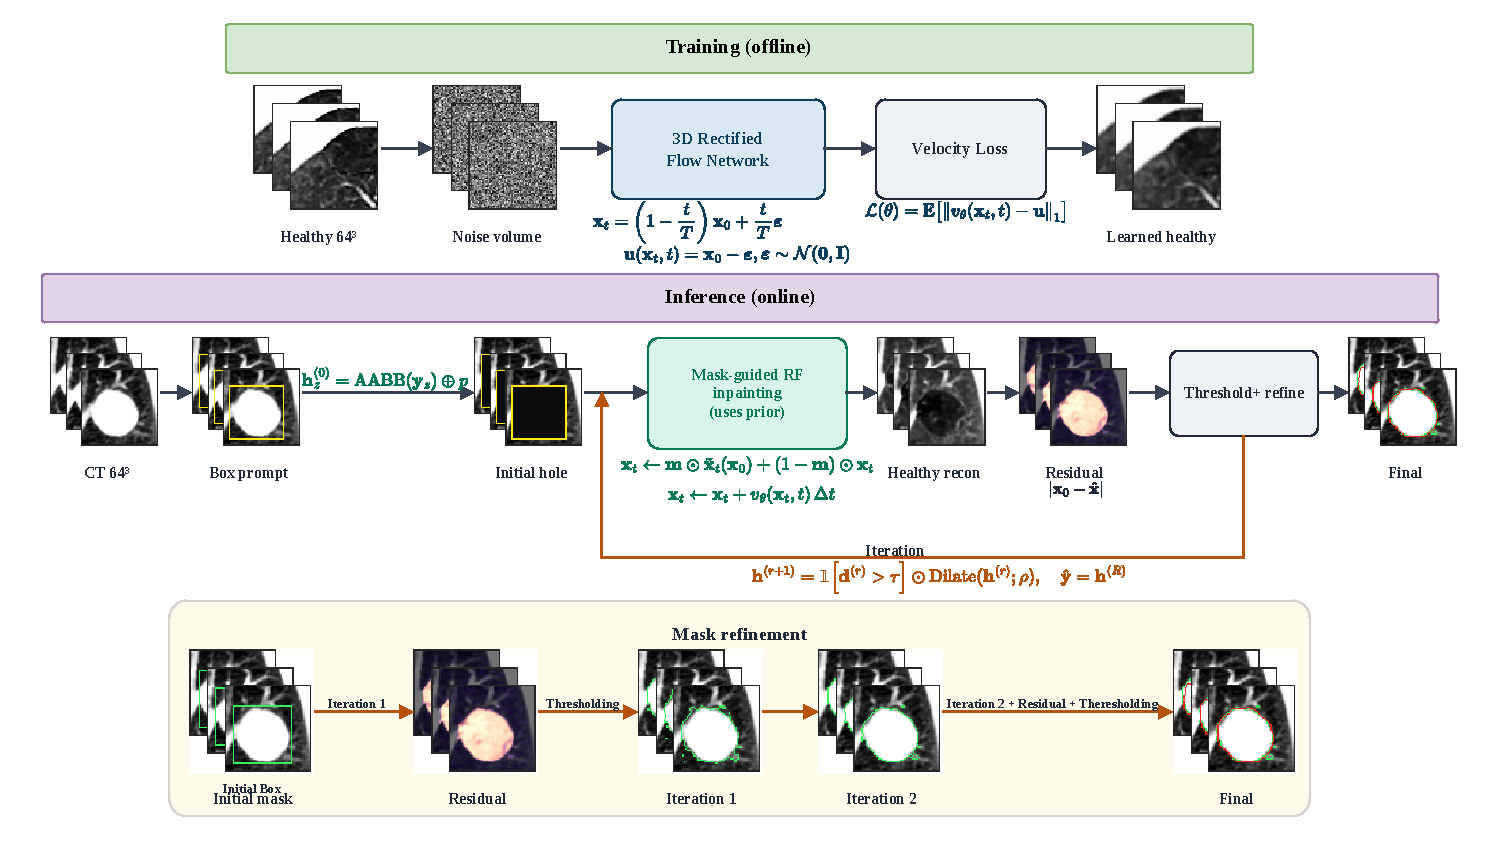
\includegraphics[width=\textwidth]{figures/bakeoff/method_overview/fig_method_overview_2.drawio.pdf}
  \caption{Method overview.
  \textbf{Top (training):} a 3D rectified-flow network learns a healthy CT
  prior from nodule-free \(64^{3}\) patches (path / velocity equations shown
  under the blocks).
  \textbf{Middle (inference):} a box prompt defines an initial hole;
  mask-guided inpainting (using the prior) produces a healthy reconstruction;
  the residual \(|\mathbf{x}_0-\hat{\mathbf{x}}|\) is thresholded and refined
  for \(R\) rounds (RF path, RePaint inject, residual, and dilation update
  shown beside the blocks).
  \textbf{Bottom:} mask refinement---initial box mask, then Iteration~1
  and Iteration~2 masks (lime contours).
  Panels show three consecutive axial slices.}
  \label{fig:method}
\end{figure*}

\paragraph{Notation.}
Let \(\mathbf{x}\in\mathbb{R}^{D\times H\times W}\) denote a CT patch after HU
windowing and normalization (Sec.~\ref{sec:method:data}).
Let \(\mathbf{y}\in\{0,1\}^{D\times H\times W}\) be the ground-truth nodule mask
(used to construct oracle box prompts for fair comparison, and for evaluation
only; deployment can use detector or user boxes).
We write \(\mathbf{m}\in\{0,1\}^{D\times H\times W}\) for the \emph{keep} mask
(\(\mathbf{m}=1\) known~/~observed, \(\mathbf{m}=0\) inpaint hole) and
\(\mathbf{h}=1-\mathbf{m}\) for the hole.
The network \(v_\theta\) predicts a rectified-flow velocity field.

%------------------------------------------------------------------------------
\subsection{Problem Formulation}
\label{sec:method:problem}
%------------------------------------------------------------------------------

Given a thoracic CT patch and a candidate region prompt, the goal is to
recover a binary segmentation \(\hat{\mathbf{y}}\) of any lesion in that region
(or an empty mask if the region is healthy).
Conventional discriminative segmenters map \(\mathbf{x}\mapsto\hat{\mathbf{y}}\)
directly.
In contrast, we leverage the observation that nodules are \emph{deviations from
healthy lung anatomy}: if a generative model of healthy tissue is forced to
reconstruct an erased nodule region, the reconstruction \(\hat{\mathbf{x}}\)
disagrees with \(\mathbf{x}\) precisely where anomalous tissue lies.
The final hole \(\mathbf{h}^\star\) obtained after residual-driven refinement
is taken as the prediction,
\begin{equation}
\hat{\mathbf{y}} \;=\; \mathbf{h}^\star.
\end{equation}

%------------------------------------------------------------------------------
\subsection{Data and Preprocessing}
\label{sec:method:data}
%------------------------------------------------------------------------------

We use LIDC-IDRI chest CT volumes~\cite{lidc2011}.
Patches of size \(64^{3}\) are extracted at resampling to spacing
\((0.7,0.7,1.5)\,\mathrm{mm}\) and retained only when the lung mask occupies at
least \(25\%\) of the patch.
Intensities are clipped to \([-1000,400]\,\mathrm{HU}\) and linearly mapped to
\([0,1]\):
\begin{equation}
\begin{aligned}
\tilde{x}
&=
\mathrm{clip}\!\Bigl(
\tfrac{x - \mathrm{HU}_{\min}}{\mathrm{HU}_{\max}-\mathrm{HU}_{\min}},\,0,1
\Bigr),\\
\mathrm{HU}_{\min}&=-1000,\qquad
\mathrm{HU}_{\max}=400.
\end{aligned}
\end{equation}
Training uses \emph{nodule-free} (healthy) patches; inference and evaluation use
\emph{positive} nodule patches with LIDC consensus annotations.
Patient-level disjoint splits prevent leakage across train~/~validation~/~test.

%------------------------------------------------------------------------------
\subsection{Healthy Tissue Prior via Rectified Flow}
\label{sec:method:rflow}
%------------------------------------------------------------------------------

\paragraph{Generative model.}
We train an unconditional 3D U-Net \(v_\theta\)~\cite{ronneberger2015unet}
to transport noise to healthy CT under
\emph{rectified flow}~\cite{liu2023flow,lipman2023flowmatching}.
Relative to score-based DDPM training~\cite{ho2020ddpm}, rectified flow learns a nearly straight
probability path between \(\boldsymbol{\varepsilon}\sim\mathcal{N}(\mathbf{0},\mathbf{I})\)
and data \(\mathbf{x}_0\), yielding efficient few-step ODE sampling.

\paragraph{Training path.}
Let \(T\) denote the continuous time horizon (we use \(T{=}1000\) with continuous
timesteps and timestep transform~\cite{esser2024sd3}), and write
\(s\coloneqq t/T\in[0,1]\) for normalized time.
Pair a healthy patch \(\mathbf{x}_0\sim p_{\mathrm{healthy}}\) with
\(\boldsymbol{\varepsilon}\sim\mathcal{N}(\mathbf{0},\mathbf{I})\) and form the
\emph{linear interpolant} with constant target velocity
\begin{equation}
\label{eq:path}
\mathbf{x}_t
=
(1-s)\,\mathbf{x}_0
+
s\,\boldsymbol{\varepsilon},
\qquad
\mathbf{u}
\;\coloneqq\;
\frac{\mathrm{d}\mathbf{x}_t}{\mathrm{d}s}
=
\mathbf{x}_0-\boldsymbol{\varepsilon}.
\end{equation}
Sampling transports noise (\(s{=}1\)) to data (\(s{=}0\)) by the ODE
\(\mathrm{d}\mathbf{x}/\mathrm{d}s=v_\theta(\mathbf{x},sT)\) with
\(\mathbf{x}|_{s=1}\sim\mathcal{N}(\mathbf{0},\mathbf{I})\).
We train \(v_\theta\) by conditional flow matching~\cite{lipman2023flowmatching}
with an \(\ell_1\) velocity objective
\begin{equation}
\label{eq:loss}
\mathcal{L}(\theta)
=
\mathbb{E}_{\mathbf{x}_0,\boldsymbol{\varepsilon},t}
\bigl[
\norm{v_\theta(\mathbf{x}_t,t)-(\mathbf{x}_0-\boldsymbol{\varepsilon})}_1
\bigr].
\end{equation}
Volumes are standardized by a fixed scale factor
\(s_{\mathrm{std}}=1/\mathrm{std}(\mathbf{x})\) estimated once from training
data (MAISI-style) and reused for training and inference; outputs are
rescaled after sampling. All ODEs below are stated in this scaled space.

\begin{proposition}[Straight-path velocity]
\label{prop:velocity}
For the interpolant in~\eqref{eq:path}, \(\mathrm{d}\mathbf{x}_t/\mathrm{d}s\)
is constantly \(\mathbf{x}_0-\boldsymbol{\varepsilon}\), with endpoints
\(\mathbf{x}_{t=0}=\mathbf{x}_0\) and \(\mathbf{x}_{t=T}=\boldsymbol{\varepsilon}\).
\end{proposition}
\begin{proof}
Differentiate~\eqref{eq:path} and substitute \(s{=}0\) and \(s{=}1\).
\end{proof}

\begin{proposition}[Exact \(x_0\) recovery]
\label{prop:x0}
If \(v_\theta(\mathbf{x}_t,t)=\mathbf{u}\) along~\eqref{eq:path}, then
\begin{equation}
\label{eq:x0hat}
\hat{\mathbf{x}}_0(\mathbf{x}_t,t)
\;\coloneqq\;
\mathbf{x}_t + s\,v_\theta(\mathbf{x}_t,t)
\end{equation}
recovers \(\mathbf{x}_0\) for every \(s\in[0,1]\).
\end{proposition}
\begin{proof}
\(\mathbf{x}_t+s(\mathbf{x}_0-\boldsymbol{\varepsilon})
=(1-s)\mathbf{x}_0+s\boldsymbol{\varepsilon}
+s\mathbf{x}_0-s\boldsymbol{\varepsilon}
=\mathbf{x}_0\).
\end{proof}

\begin{corollary}[Flow-matching fixed point]
\label{cor:fm}
Any zero-risk minimizer of~\eqref{eq:loss} has characteristics given by the
rectified straight paths of Liu~et~al.~\cite{liu2023flow}.
Euler integration from \(s{=}1\) to \(s{=}0\) then maps
\(\boldsymbol{\varepsilon}\) to \(\mathbf{x}_0\) in one analytic step when
\(v_\theta\) is exact, and in \(N\) discrete steps otherwise.
\end{corollary}

\paragraph{Network and training regime.}
The velocity field is a compact single-channel 3D U-Net over \(64^{3}\)
patches: capacity is spent on local parenchyma texture rather than
long-range attention, and spatial self-attention is disabled.
Crucially, training is \emph{unconditional}: no boxes, lesion masks, or
ControlNet-style side inputs are provided, so \(v_\theta\) learns only
what healthy lung looks like.
Mild flips and intensity jitter regularize the prior without introducing
lesion-like contrast that would contaminate residual scoring at inference.
Full channel widths and optimizer settings are listed in
Table~\ref{tab:hparams} (Supplementary Material).

%------------------------------------------------------------------------------
\subsection{Mask-Guided Rectified-Flow Inpainting}
\label{sec:method:repaint}
%------------------------------------------------------------------------------

At inference we are given an observation \(\mathbf{x}_0\) and a keep-mask
\(\mathbf{m}\) (\(\mathbf{m}=1\) observed, \(\mathbf{m}=0\) hole).
Write \(\mathcal{K}=\{\,i:m_i=1\,\}\) and \(\mathcal{H}=\{\,i:m_i=0\,\}\)
for known and hole index sets.
We seek a healthy counterfactual \(\hat{\mathbf{x}}\) that
(i)~agrees with \(\mathbf{x}_0\) on \(\mathcal{K}\) and
(ii)~is drawn from the learned healthy flow on \(\mathcal{H}\).

\paragraph{Inject and constrained Euler sampling.}
Let \(\tilde{\mathbf{x}}_t(\mathbf{x}_0)\) denote the forward interpolant
of~\eqref{eq:path} with a fresh noise draw
\(\boldsymbol{\varepsilon}'\sim\mathcal{N}(\mathbf{0},\mathbf{I})\).
Following RePaint~\cite{lugmayr2022repaint}, but without jump resampling,
known voxels are overwritten at each reverse time \(t\) by
\begin{equation}
\label{eq:inject}
\mathbf{x}_t
\;\leftarrow\;
\mathbf{m}\odot\tilde{\mathbf{x}}_t(\mathbf{x}_0)
\;+\;
(1-\mathbf{m})\odot\mathbf{x}_t.
\end{equation}
Sampling starts from \(\mathbf{x}_{t_1}\sim\mathcal{N}(\mathbf{0},\mathbf{I})\)
on a decreasing schedule
\(T\approx t_1>t_2>\cdots>t_N\approx 0\)
(\(N{=}40\) by default). For \(k=1,\dots,N-1\) we apply inject
then an Euler step,
\begin{equation}
\label{eq:sampler}
\begin{aligned}
\mathbf{x}_{t_k}
&\;\leftarrow\;
\mathbf{m}\odot\tilde{\mathbf{x}}_{t_k}(\mathbf{x}_0)
+(1-\mathbf{m})\odot\mathbf{x}_{t_k},\\
\mathbf{x}_{t_{k+1}}
&\;\leftarrow\;
\mathbf{x}_{t_k}
+
v_\theta(\mathbf{x}_{t_k},t_k)\,\Delta s_k,
\qquad
\Delta s_k=\tfrac{t_k-t_{k+1}}{T}.
\end{aligned}
\end{equation}
After unscaling we set \(\hat{\mathbf{x}}\coloneqq\mathbf{x}_{t_N}\) and write
\(\hat{\mathbf{x}}=\mathcal{G}_\theta(\mathbf{x}_0,\mathbf{m})\) for the full
mask-guided inpainting map.

\begin{proposition}[Known-region marginal consistency]
\label{prop:inject}
Fix \(\mathbf{x}_0\) and \(\mathbf{m}\).
After each application of~\eqref{eq:inject}, the restriction
\(\mathbf{x}_t\big|_{\mathcal{K}}\) equals the forward interpolant of
\(\mathbf{x}_0\big|_{\mathcal{K}}\) at time \(t\), independent of the free
evolution on \(\mathcal{H}\).
\end{proposition}
\begin{proof}
On \(i\in\mathcal{K}\),~\eqref{eq:inject} replaces the state by
\(\tilde{x}_{t,i}(\mathbf{x}_0)=(1-s)x_{0,i}+s\varepsilon'_i\).
Coordinates in \(\mathcal{H}\) are unchanged by the inject.
\end{proof}

\begin{proposition}[Exact reverse step along a path]
\label{prop:euler}
If \(v_\theta=\mathbf{u}\) from~\eqref{eq:path} and \(\mathbf{x}_{t_k}\)
lies on the interpolant of some pair
\((\mathbf{x}_0^\star,\boldsymbol{\varepsilon})\), then the Euler update
in~\eqref{eq:sampler} lands exactly on the same interpolant at time
\(t_{k+1}\).
\end{proposition}
\begin{proof}
With \(s_k=t_k/T\) and \(\Delta s_k=s_k-s_{k+1}\),
\begin{align*}
\mathbf{x}_{t_k}+\Delta s_k\,(\mathbf{x}_0^\star-\boldsymbol{\varepsilon})
&=
(1-s_k)\mathbf{x}_0^\star+s_k\boldsymbol{\varepsilon}
+(s_k-s_{k+1})\bigl(\mathbf{x}_0^\star-\boldsymbol{\varepsilon}\bigr)\\
&=
(1-s_{k+1})\mathbf{x}_0^\star+s_{k+1}\boldsymbol{\varepsilon}.
\end{align*}
\end{proof}

\begin{corollary}[Boundary-consistent healthy fill]
\label{cor:inpaint}
Under Propositions~\ref{prop:inject}--\ref{prop:euler} with an exact
velocity field,
\(\hat{\mathbf{x}}\big|_{\mathcal{K}}=\mathbf{x}_0\big|_{\mathcal{K}}\)
(up to the final \(s{=}0\) inject), while
\(\hat{\mathbf{x}}\big|_{\mathcal{H}}\) is a healthy draw conditioned on
the observed context.
\end{corollary}

Thus inject anchors the reverse process on \(\mathcal{K}\), and the healthy
velocity fills \(\mathcal{H}\), yielding a \emph{healthy counterfactual} of
\(\mathbf{x}_0\) under the box prompt.

%------------------------------------------------------------------------------
\subsection{Initial Hole from Slice-wise Boxes}
\label{sec:method:init}
%------------------------------------------------------------------------------

Prompted methods require a spatial query.
Following standard interactive segmentation practice, we construct an
\emph{initial} hole from per-slice axis-aligned boxes of the nodule annotation
(or, at deployment, of a coarse detector or user boxes).
For each axial slice \(z\) containing foreground,
\begin{equation}
\mathbf{h}^{(0)}_z
=
\mathrm{AABB}_{2\mathrm{D}}\!\bigl(\mathbf{y}_z\bigr)
\oplus\, p,
\end{equation}
with padding \(p{=}2\) voxels, stacked over \(z\) into a 3D binary hole
\(\mathbf{h}^{(0)}\).
This deliberately over-covers the lesion and provides a conservative starting
region for refinement.

%------------------------------------------------------------------------------
\subsection{Iterative Residual Mask Refinement}
\label{sec:method:refine}
%------------------------------------------------------------------------------

A fixed initial hole is imperfect: it may include healthy soft tissue or miss
irregular lesion boundaries.
We therefore iterate inpainting and residual thresholding
(Algorithm~\ref{alg:refine}).

After inpainting with keep-mask \(\mathbf{m}^{(r)}=1-\mathbf{h}^{(r)}\),
\begin{equation}
\label{eq:residual}
\hat{\mathbf{x}}^{(r)}
=
\mathcal{G}_\theta\!\bigl(\mathbf{x}_0,\mathbf{m}^{(r)}\bigr),
\qquad
\mathbf{d}^{(r)}
=
\bigl|\mathbf{x}_0-\hat{\mathbf{x}}^{(r)}\bigr|.
\end{equation}
Large residuals indicate tissue that the healthy prior cannot explain.
The next hole thresholds the residual inside a dilated search band,
\begin{equation}
\label{eq:update}
\mathbf{h}'
=
\mathbb{1}\!\bigl[\mathbf{d}^{(r)}>\tau\bigr]
\;\odot\;
\mathrm{Dilate}\!\bigl(\mathbf{h}^{(r)};\,\rho\bigr),
\qquad
\mathbf{h}^{(r+1)}
=
\begin{cases}
\mathbf{h}' & \text{if }\|\mathbf{h}'\|_0\ge\eta,\\
\mathbf{h}^{(r)} & \text{otherwise,}
\end{cases}
\end{equation}
with \(\tau{=}0.05\), dilation radius \(\rho{=}2\), and stability floor
\(\eta{=}8\) voxels.
We run \(R\) refinement updates (\(R{=}2\) by default; \(R{=}3\) in
ablations) and therefore \(R{+}1\) inpaint passes: the final prediction is
the hole used for the last inpaint, \(\hat{\mathbf{y}}=\mathbf{h}^{(R)}\)
(Algorithm~\ref{alg:refine}).
No morphological open~/~close post-processing is applied in the default method.

\begin{algorithm}[t]
\caption{Iterative residual mask refinement for nodule localization}
\label{alg:refine}
\begin{algorithmic}[1]
\REQUIRE CT patch $\mathbf{x}_0$, initial hole $\mathbf{h}^{(0)}$, RF
inpainter $\mathcal{G}_\theta$, rounds $R$, threshold $\tau$, dilation
$\rho$, min.\ voxels $\eta$
\ENSURE Predicted nodule mask $\hat{\mathbf{y}}=\mathbf{h}^{(R)}$
\FOR{$r = 0$ \TO $R$}
\STATE $\mathbf{m}^{(r)} \gets 1-\mathbf{h}^{(r)}$
\STATE $\hat{\mathbf{x}}^{(r)} \gets \mathcal{G}_\theta\!\bigl(
  \mathbf{x}_0,\,\mathbf{m}^{(r)}\bigr)$
  \COMMENT{Eqs.~\eqref{eq:inject},~\eqref{eq:sampler}}
\IF{$r = R$}
\STATE \textbf{break}
  \COMMENT{final inpaint; no further update}
\ENDIF
\STATE $\mathbf{d}^{(r)} \gets \bigl|\mathbf{x}_0-\hat{\mathbf{x}}^{(r)}\bigr|$
  \COMMENT{Eq.~\eqref{eq:residual}}
\STATE $\mathbf{b}^{(r)} \gets \mathrm{Dilate}\!\bigl(\mathbf{h}^{(r)};\,\rho\bigr)$
\STATE $\mathbf{h}' \gets \mathbb{1}\!\bigl[\mathbf{d}^{(r)}>\tau\bigr]
  \odot \mathbf{b}^{(r)}$
  \COMMENT{Eq.~\eqref{eq:update}}
\IF{$\|\mathbf{h}'\|_0 \ge \eta$}
\STATE $\mathbf{h}^{(r+1)} \gets \mathbf{h}'$
\ELSE
\STATE $\mathbf{h}^{(r+1)} \gets \mathbf{h}^{(r)}$
  \COMMENT{stability safeguard}
\ENDIF
\ENDFOR
\STATE \textbf{return} $\hat{\mathbf{y}} \gets \mathbf{h}^{(R)}$
\end{algorithmic}
\end{algorithm}

The loop couples a geometric box prior with an appearance test against the
healthy flow:~\eqref{eq:inject}--\eqref{eq:sampler} keep each inpaint
anchored to observed context, while~\eqref{eq:update} shrinks over-complete
holes toward residual-supported lesion voxels.

%------------------------------------------------------------------------------
\subsection{Relation to Discriminative and Promptable Segmenters}
\label{sec:method:discuss}
%------------------------------------------------------------------------------

Discriminative segmenters and foundation models (e.g.,
SAM-Med2D~\citep{sam_med2d2023}) map prompts to masks in a single feed-forward
pass.
Our method instead \emph{tests} a spatial hypothesis against a generative
healthy prior and updates the hypothesis via reconstruction error.
The same initial boxes used to prompt interactive models initialize our hole;
refinement then specializes the region without requiring paired nodule-dense
training of a segmenter.
This makes the approach complementary to promptable models and attractive when
healthy tissue is abundant but curated lesion masks are scarce.

%------------------------------------------------------------------------------
\subsection{Implementation Details}
\label{sec:method:impl}
%------------------------------------------------------------------------------

Unless noted otherwise we use \(N{=}40\) RF inference steps, \(R{=}2\)
refinement rounds, \(\tau{=}0.05\), \(\rho{=}2\), and \(p{=}2\).
Checkpoints are selected by validation velocity loss on held-out healthy
patches.
All experiments share the same HU normalization and \(64^{3}\) geometry as
training.
We report mean Dice and IoU between \(\hat{\mathbf{y}}\) and LIDC nodule
masks on a held-out positive-patch test set (precision/recall are computed
but not tabulated).

Ablations over \(N\in\{30,40,60,80\}\) and \(R\in\{2,3\}\) are reported in
Section~\ref{sec:experiments}; the default LIDC operating point uses
\(N{=}40\) and \(R{=}2\).

% =============================================================
\section{Experiments}
\label{sec:experiments}

We evaluate region-prompted anomaly verification against
interactive foundation segmenters under \emph{matched box
prompts}. The primary questions are: (i)~when a true nodule is
present, how well do we recover it? and (ii)~when the prompted
region is healthy, how often do models still produce a spurious
mask? We answer (i)--(ii) on LIDC first, then test whether the
same trends hold on MAISI and NSCLC, and finally ablate inference
compute for Ours.

\subsection{Datasets and Protocol}
\paragraph{Positive LIDC hold-out.}
We evaluate on a patient-disjoint test cache of \(N{=}1658\) nodule-centered
\(64^3\) patches from LIDC-IDRI~\citep{lidc2011}, resampled to
\(0.7{\times}0.7{\times}1.5\,\mathrm{mm}\) and intensity-windowed to
\([-1000,400]\)~HU (same preprocessing as Section~\ref{sec:method:data}).
Radiologist consensus masks are used \emph{only for evaluation}.

\paragraph{Additional positive sets.}
Under the same matched-box protocol we also evaluate
MAISI synthetic nodule patches~\citep{maisi2025} (\(N{=}109\) patches) and
NSCLC-Radiomics~\citep{aerts2014nsclc} (\(N{=}85\) full GTV volumes,
inferred by overlapping \(64^{3}\) tiles that are stitched back to the volume;
qualitative figures additionally show matched \(64^{3}\) crops).
All methods use the same prompts and the same pretrained healthy-prior
checkpoint for Ours; only RF inference settings (steps / refine rounds \(R\))
are dataset-specific, as noted in Table~\ref{tab:cross}.

\paragraph{Prompting.}
All methods receive identical per-slice 2D bounding boxes derived from the
nodule / GTV mask with \(2\)-voxel padding (our ``Strategy-4'' box cue).
Ours converts these boxes into an inpainting hole; interactive baselines
consume them as box prompts.

\paragraph{Healthy false-positive probe.}
To measure over-segmentation on normal tissue, we place random boxes inside
\emph{nodule-free} LIDC lung patches (\(N{=}3840\) prompts) and report
\emph{mean predicted mask volume} (mm\(^3\)). Because the ground truth is
empty, we do not report Dice against an empty mask.

\subsection{Baselines}
We compare against interactive models that accept the same box interface:
SAM-Med2D~\citep{sam_med2d2023},
SAM-Med3D~\citep{sam_med3d2023},
SegVol~\citep{segvol2024},
VISTA3D~\citep{vista3d2024}, and
nnInteractive~\citep{nninteractive2025}.
For Ours we report a rectified-flow checkpoint with iterative residual
refinement. Unless stated otherwise, the default LIDC configuration is
\(40\) inference steps and \(R{=}2\) refine rounds; healthy-FP and
cross-dataset tables note any alternate settings used for reporting.

\subsection{Main Results on LIDC}
\label{sec:exp:lidc}
Table~\ref{tab:main} reports matched-box true-nodule Dice~/~IoU
(\(N{=}1658\)) together with healthy false-positive predicted volume
(\(N{=}3840\) random boxes in nodule-free lung).
Ours is nearly tied with the strongest interactive baseline
(SAM-Med2D; both round to Dice \(0.73\), with SAM-Med2D slightly ahead before
rounding) and ahead of nnInteractive, SAM-Med3D, SegVol, and VISTA3D, despite
never training on lesion masks.
Among methods that remain competitive on true nodules, the recommended
Ours configuration (\(40\)-step, \(R{=}2\)) yields substantially less
spurious volume than SAM-Med2D~\citep{sam_med2d2023}, SegVol, and especially
nnInteractive~\citep{nninteractive2025}; a \(60\)-step/\(R{=}3\) setting
further reduces FP volume.
VISTA3D~\citep{vista3d2024} is nearly silent on healthy tissue, but its
LIDC Dice (\(0.19\)) shows that silence alone is not useful without
sensitivity to real nodules.
Figure~\ref{fig:results} summarizes the same comparison;
Figure~\ref{fig:fp-tradeoff} places every method in the true-nodule Dice
vs.\ healthy FP volume plane.

\begin{table*}[t]
\centering
\caption{LIDC matched-box evaluation: true-nodule Dice~/~IoU
(\(N{=}1658\) positive patches) and healthy false-positive predicted
volume (\(N{=}3840\) nodule-free prompts). Best Dice~/~IoU and lowest
non-silent FP volume in \textbf{bold}. Dice against empty GT is omitted.}
\label{tab:main}
\label{tab:healthy_fp}
\begin{tabular}{lcccc}
\toprule
Method & Prompt & Dice \(\uparrow\) & IoU \(\uparrow\) &
Pred.\ vol.\ (mm\(^3\)) \(\downarrow\) \\
\midrule
SAM-Med2D
  & Box & \textbf{0.73} & \textbf{0.60} & 1980 \\
\textbf{Ours (40-step, \(R{=}2\))}
  & Box & \textbf{0.73} & 0.59 & 1076 \\
Ours (40-step, \(R{=}3\))
  & Box & 0.72 & 0.59 & --- \\
Ours (60-step, \(R{=}3\))
  & Box & --- & --- & \textbf{1006} \\
nnInteractive
  & Box & 0.71 & 0.58 & 4015 \\
SAM-Med3D
  & Box & 0.54 & 0.40 & 2872 \\
SegVol
  & Box & 0.37 & 0.25 & 1395 \\
VISTA3D$^\dagger$
  & Box & 0.19 & 0.11 & \(0\) \\
\bottomrule
\end{tabular}\\[0.25em]
{\footnotesize $^\dagger$Near-silent on healthy prompts, but poor on
true nodules.}
\end{table*}

\paragraph{Takeaway.}
On true nodules, healthy-counterfactual inpainting matches strong
2D interactive segmentation and is competitive with or stronger than
the native-3D promptable models under the same boxes, while remaining
more conservative on healthy random boxes
(Table~\ref{tab:main}).
Figure~\ref{fig:qual-lidc} shows matched box-prompt predictions on
selected LIDC cases with high Ours--GT agreement; under the same
prompts, SAM-Med2D can under-segment, nnInteractive can inflate toward
the box, and SegVol / VISTA3D can leave incomplete masks.

\begin{figure*}[t]
  \centering
  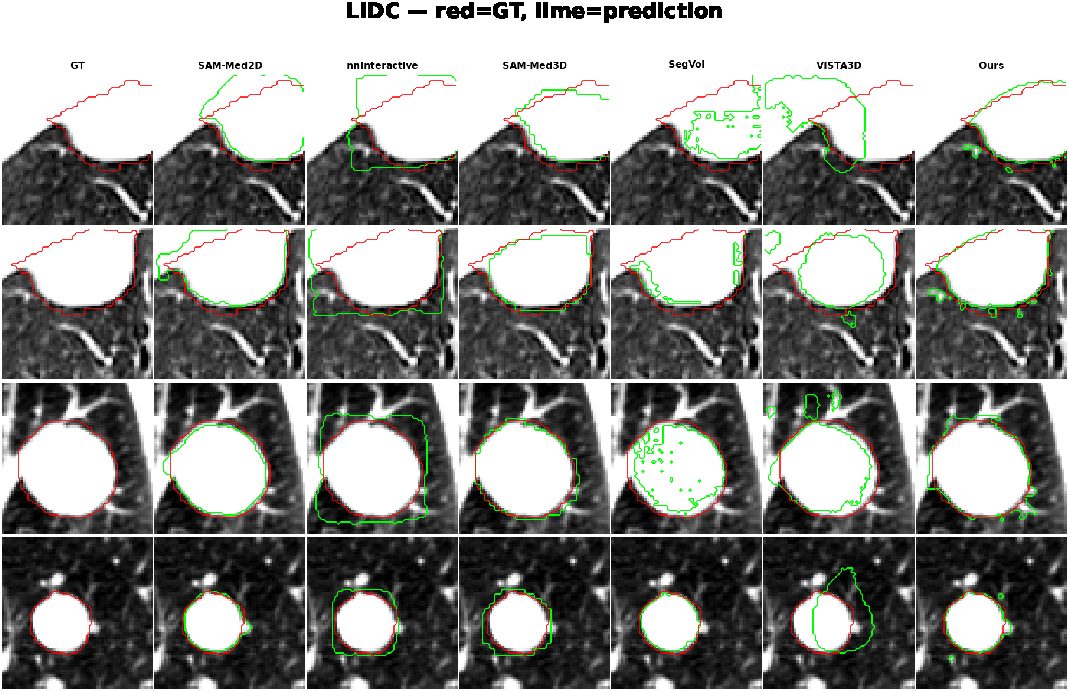
\includegraphics[width=\textwidth]{figures/fig_qual_lidc.pdf}
  \caption{Qualitative LIDC overlays under matched box prompts
  (red~=~GT, lime~=~prediction). Columns: GT, SAM-Med2D, nnInteractive,
  SAM-Med3D, SegVol, VISTA3D, and Ours. Ours uses \(40\) steps and
  \(R{=}2\). Cases shown are high-agreement examples under the same prompts.}
  \label{fig:qual-lidc}
\end{figure*}

\begin{figure}[t]
  \centering
  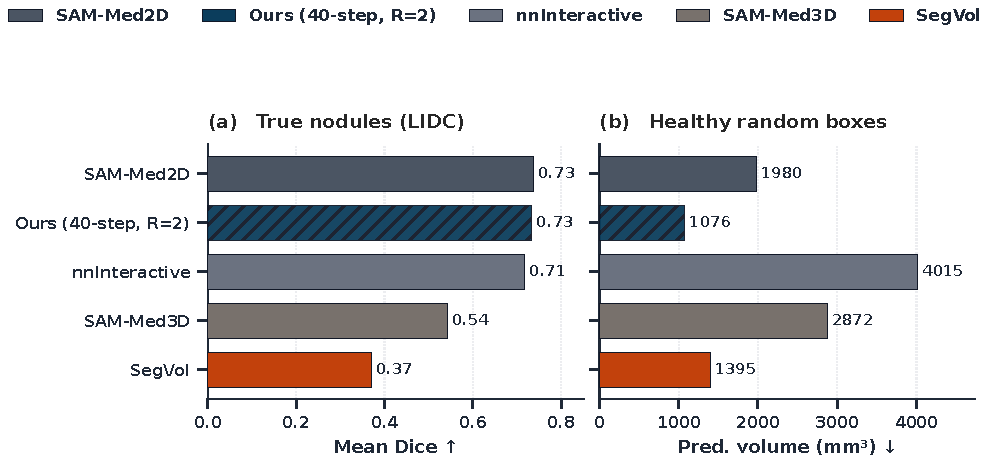
\includegraphics[width=\linewidth]{figures/fig_results_bars.pdf}
  \caption{Matched box prompts: (a)~LIDC Dice on true nodules;
  (b)~predicted volume on healthy random boxes (shared method order).
  Ours is nearly tied with SAM-Med2D on (a) while producing
  substantially less spurious mass on (b).}
  \label{fig:results}
\end{figure}

\begin{figure}[t]
  \centering
  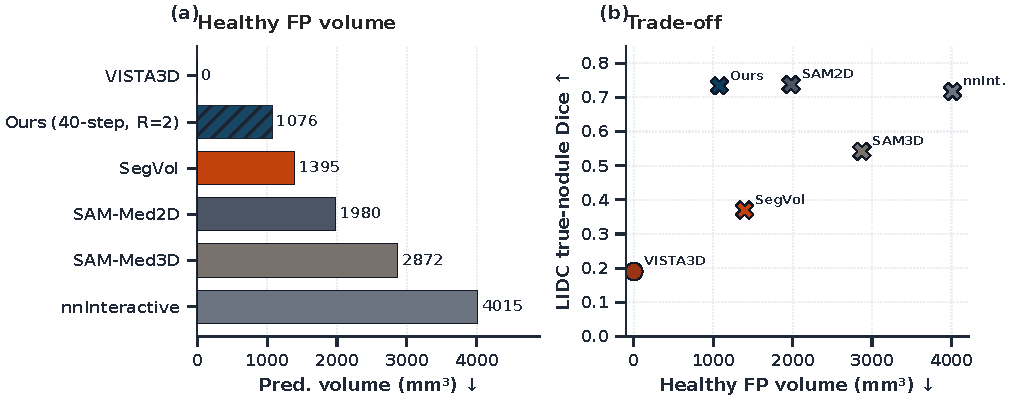
\includegraphics[width=\linewidth]{figures/fig_healthy_fp_tradeoff.pdf}
  \caption{Healthy FP probe trade-off: (a)~mean predicted volume;
  (b)~LIDC true-nodule Dice vs.\ healthy FP volume. Silent models
  (e.g., VISTA3D) sit at zero volume but low positive Dice.}
  \label{fig:fp-tradeoff}
\end{figure}

\paragraph{Takeaway.}
Interactive segmenters optimize objectness inside the box and often
over-segment healthy parenchyma under this probe. Under the same prompts,
the healthy-prior model is more conservative: competitive Dice when an
anomaly is present, and less spurious predicted volume when it is not
(Table~\ref{tab:healthy_fp}).
Figure~\ref{fig:qual-fp} illustrates empty-GT random boxes where
SAM-Med2D / SAM-Med3D / SegVol often paint lime masks inside the prompt,
whereas Ours remains sparse.

\begin{figure*}[t]
  \centering
  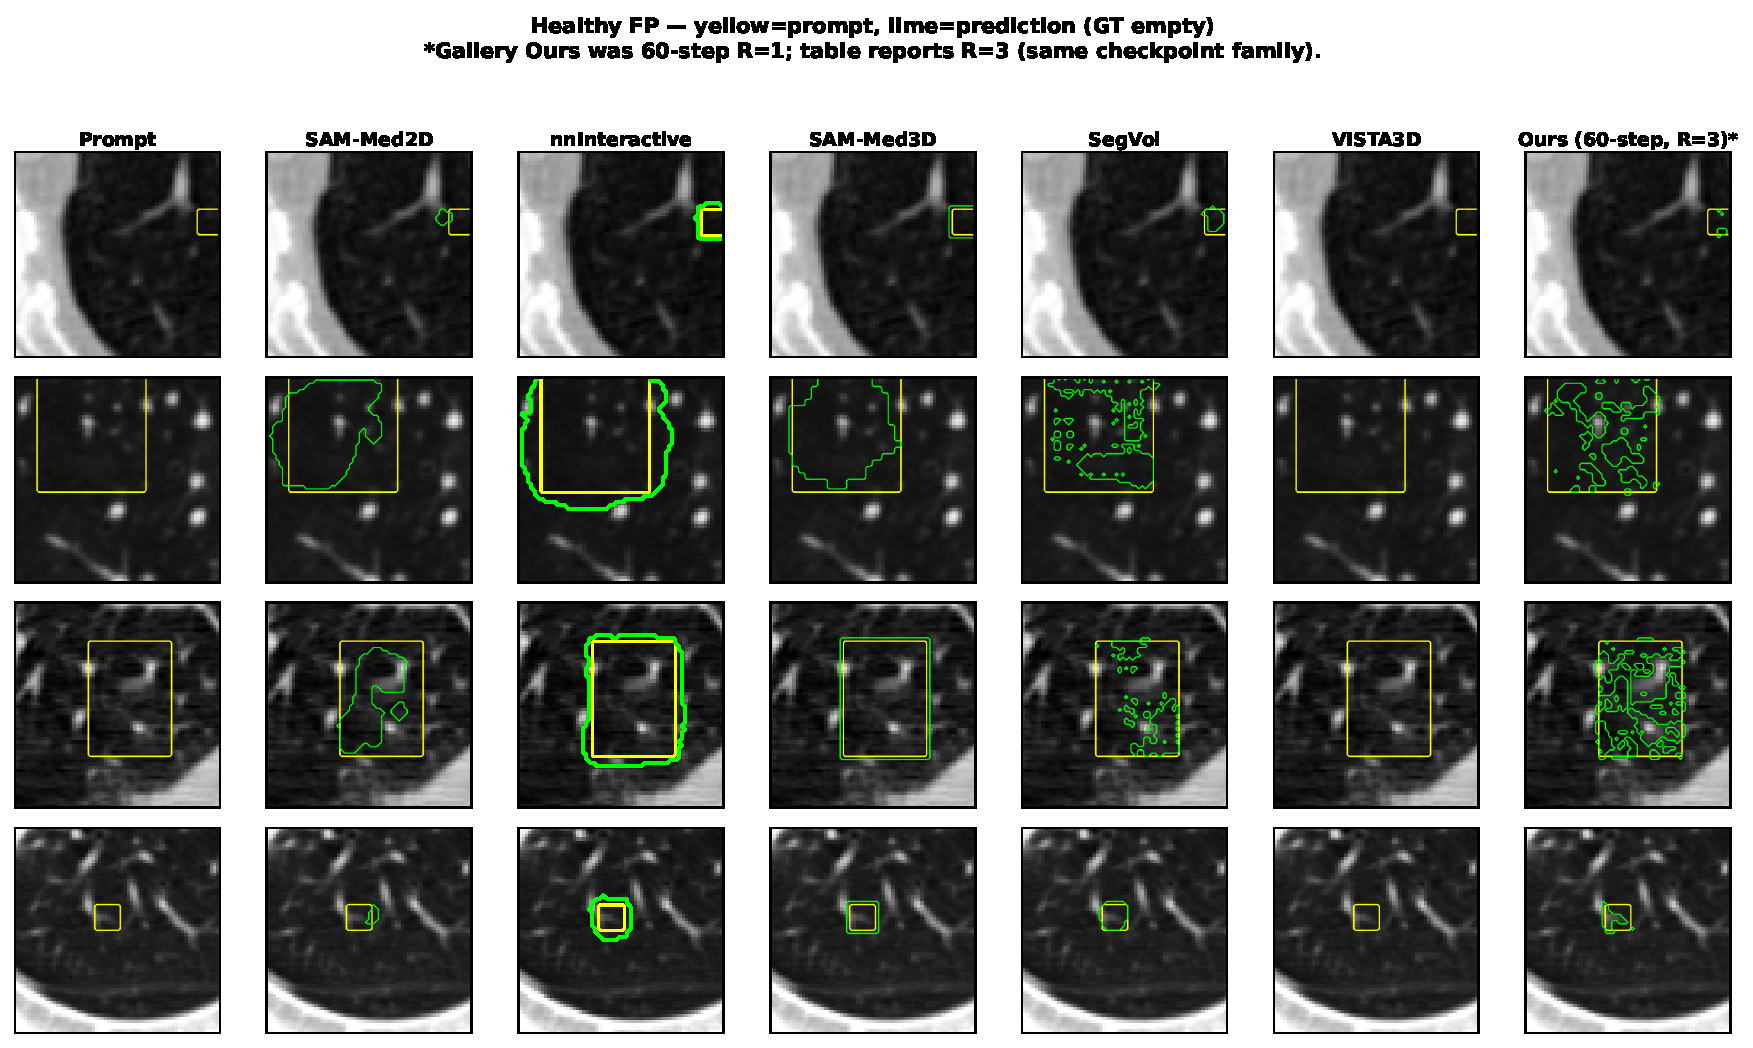
\includegraphics[width=\textwidth]{figures/fig_qual_healthy_fp.pdf}
  \caption{Healthy false-positive probe: random boxes in nodule-free
  lung (yellow~=~prompt contour, green~=~predicted mask fill; GT empty).
  Columns match Figure~\ref{fig:qual-lidc}. Object-centric baselines often
  fill the box; Ours (\(60\)-step, \(R{=}3\); Table~\ref{tab:healthy_fp})
  is more conservative.}
  \label{fig:qual-fp}
\end{figure*}

\subsection{Generalization: MAISI and NSCLC}
Table~\ref{tab:cross} and Figures~\ref{fig:bench}--\ref{fig:bench-per}
report mean Dice under the same matched-box protocol on
MAISI~\citep{maisi2025} and NSCLC-Radiomics~\citep{aerts2014nsclc},
with LIDC repeated for reference. Ours remains in a competitive tier on
all three sets (MAISI: \(60\)-step, \(R{=}3\); NSCLC: \(60\)-step,
\(R{=}1\)): within rounding of nnInteractive on MAISI (both \(0.71\) at
two decimals; nnInteractive slightly higher before rounding) and within
\(0.01\) Dice of the best NSCLC entry (\(0.78\) vs.\ \(0.79\)).
Figure~\ref{fig:qual-cross} shows corresponding overlays on MAISI
synthetic nodules and matched NSCLC \(64^3\) tumor patches;
Figure~\ref{fig:qual-nsclc-vol} shows the same four NSCLC cases as
full-volume slices. The qualitative pattern is consistent with the
tables under matched boxes, suggesting the healthy-prior residual is
not an LIDC-only artifact.

\begin{table}[t]
\centering
\caption{Mean Dice under matched box prompts across datasets.
Ours uses \(40\)-step/\(R{=}2\) on LIDC, \(60\)-step/\(R{=}3\) on
MAISI, and \(60\)-step/\(R{=}1\) on NSCLC. Best per column in
\textbf{bold}.}
\label{tab:cross}
\begin{tabular}{lccc}
\toprule
Method & LIDC & MAISI & NSCLC \\
\midrule
SAM-Med2D     & \textbf{0.73} & 0.70 & 0.76 \\
Ours          & \textbf{0.73} & \textbf{0.71} & 0.78 \\
nnInteractive & 0.71 & \textbf{0.71} & \textbf{0.79} \\
SAM-Med3D     & 0.54 & 0.56 & 0.55 \\
SegVol        & 0.37 & 0.28 & 0.17 \\
VISTA3D       & 0.19 & 0.45 & 0.12 \\
\bottomrule
\end{tabular}
\end{table}

\begin{figure*}[t]
  \centering
  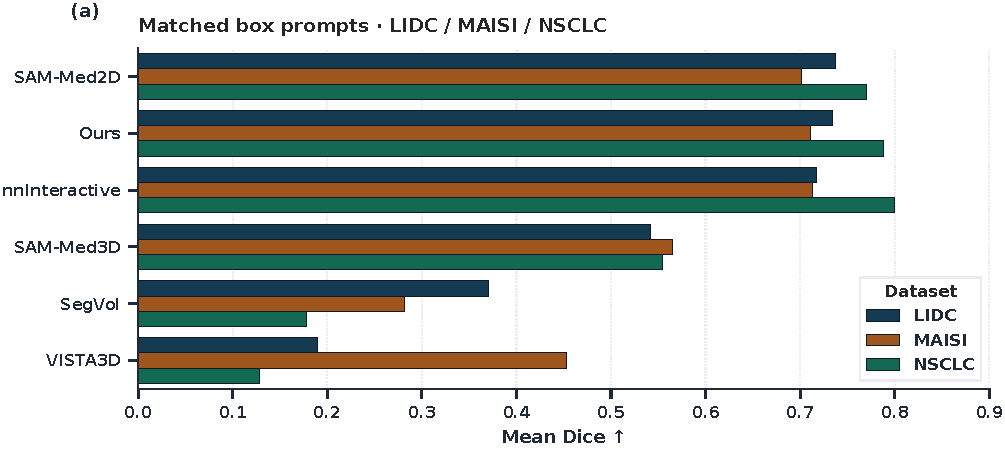
\includegraphics[width=\textwidth]{figures/fig_benchmark_dice_3datasets.pdf}
  \caption{Mean Dice under matched box prompts on LIDC, MAISI, and
  NSCLC (grouped by method). Hatched bars highlight Ours.}
  \label{fig:bench}
\end{figure*}

\begin{figure}[t]
  \centering
  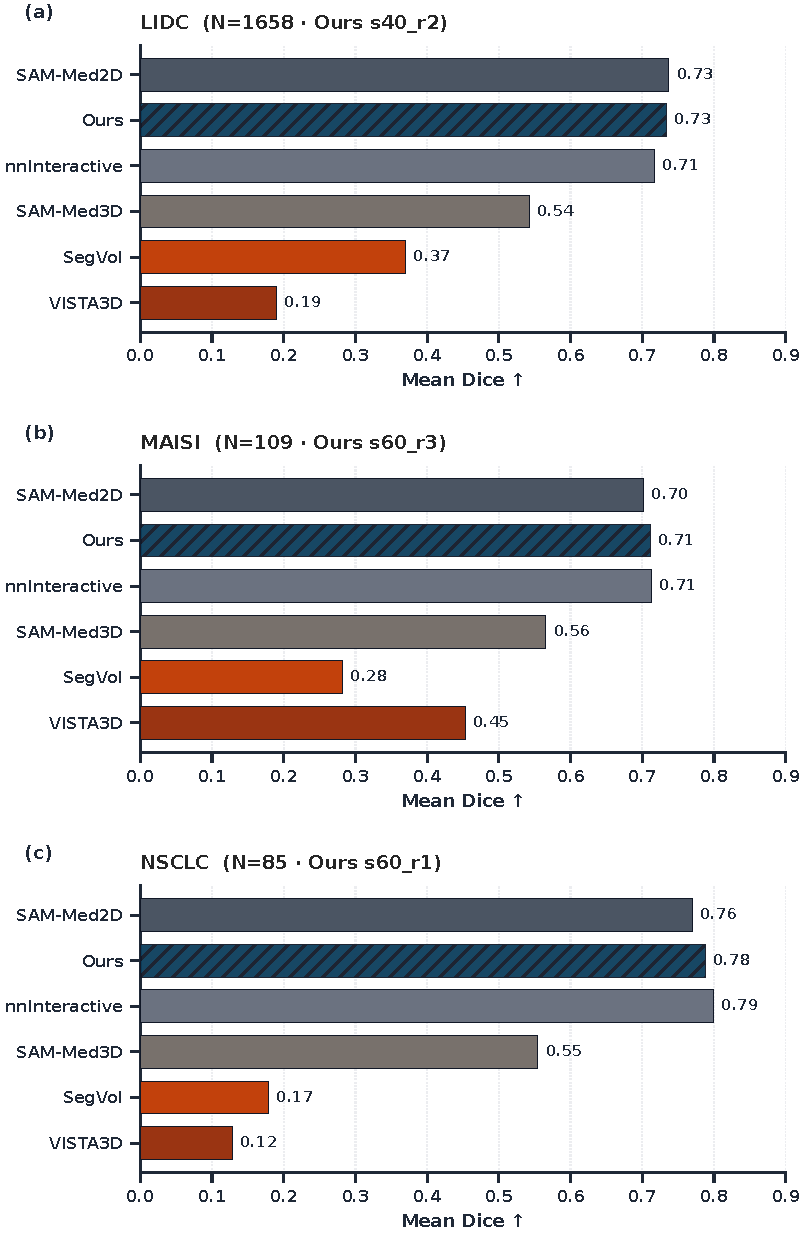
\includegraphics[width=\linewidth]{figures/fig_benchmark_dice_per_dataset.pdf}
  \caption{Per-dataset Dice under the same matched box prompts
  (LIDC, MAISI, NSCLC). Ours uses dataset-specific RF configs.}
  \label{fig:bench-per}
\end{figure}

\begin{figure*}[t]
  \centering
  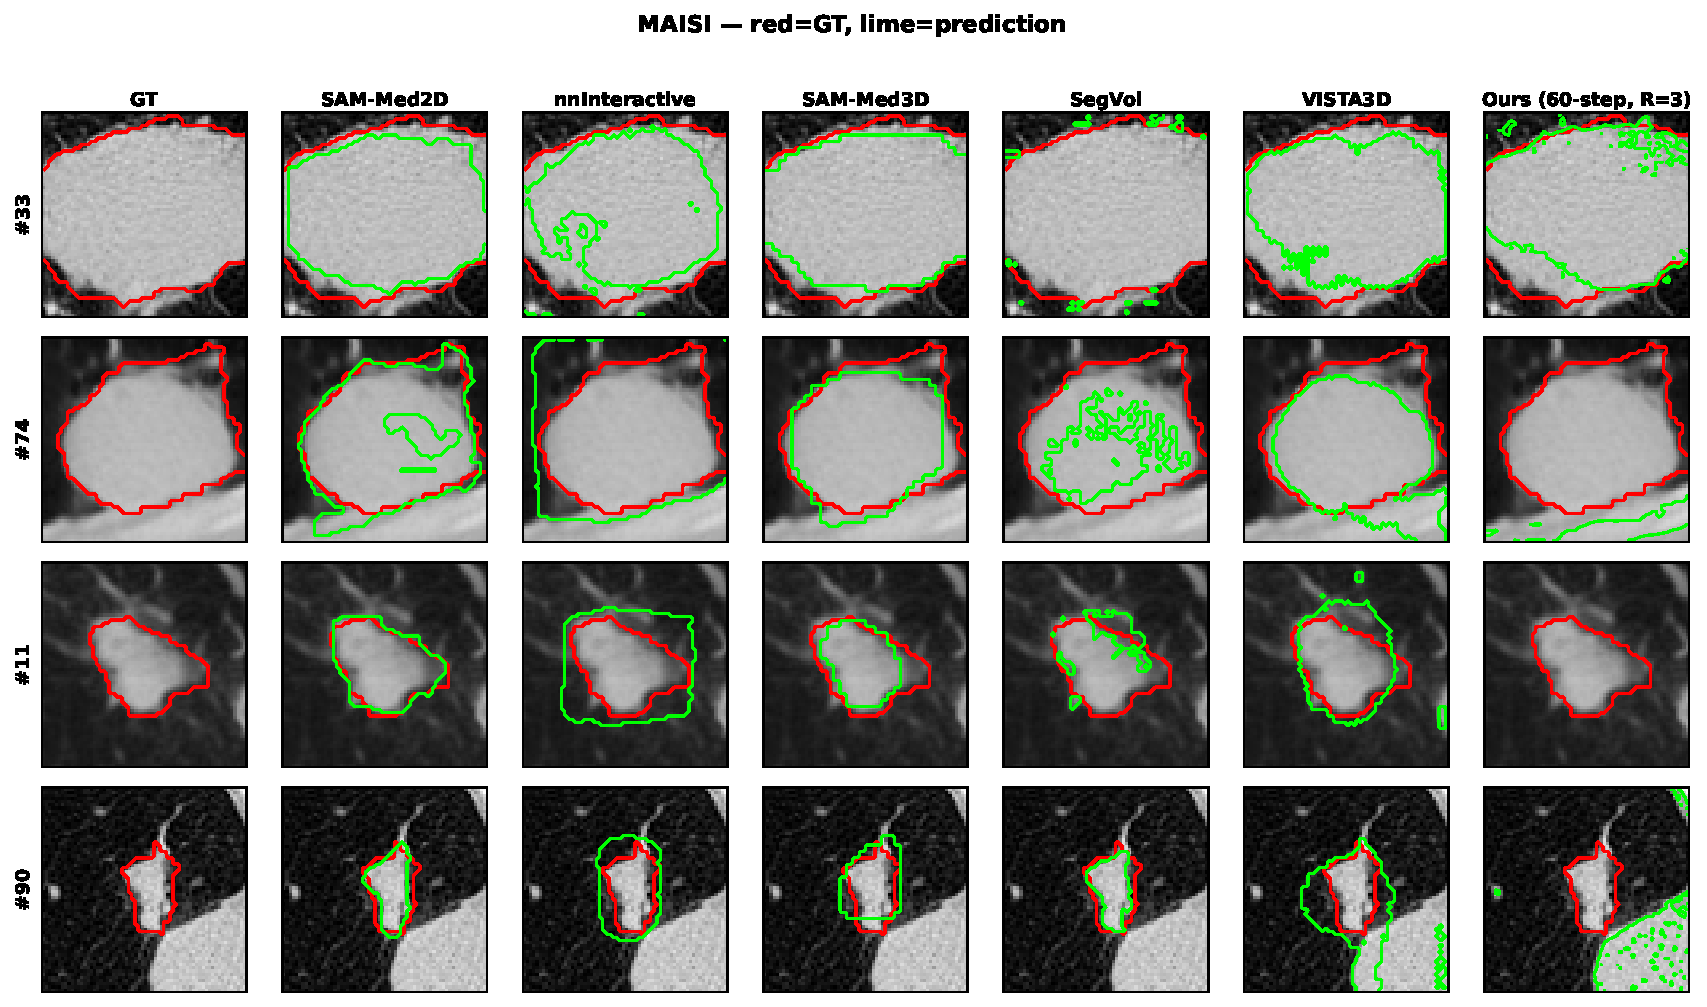
\includegraphics[width=\textwidth]{figures/fig_qual_maisi.pdf}\\[0.12em]
  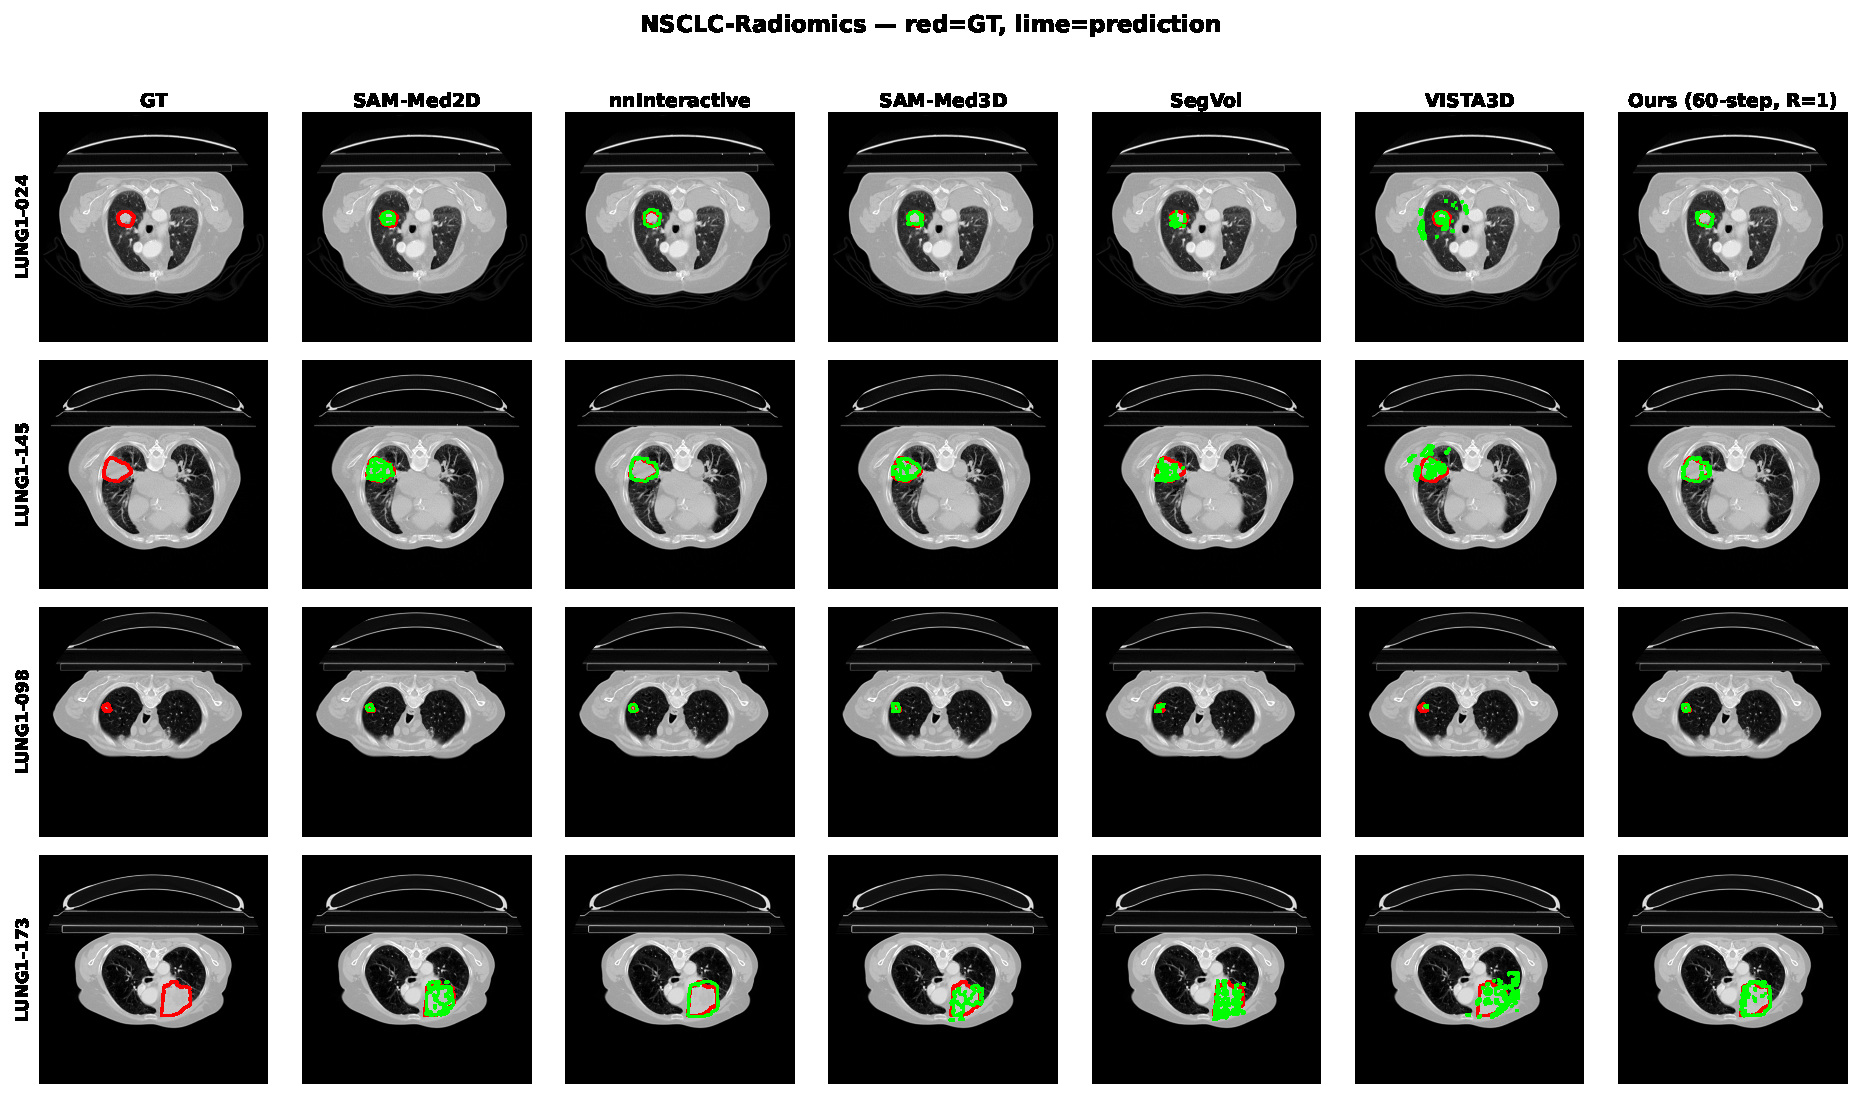
\includegraphics[width=\textwidth]{figures/fig_qual_nsclc.pdf}
  \caption{Cross-dataset qualitative overlays (red~=~GT, lime~=~prediction).
  Columns: GT, SAM-Med2D, nnInteractive, SAM-Med3D, SegVol, VISTA3D, Ours.
  Top: MAISI synthetic nodules (Ours \(60\)-step, \(R{=}3\)).
  Bottom: NSCLC-Radiomics \(64^3\) tumor patches (Ours \(60\)-step, \(R{=}1\);
  cases LUNG1-024 / 145 / 098 / 173).
  Illustrative examples under matched boxes; see Table~\ref{tab:cross}
  for aggregate Dice.}
  \label{fig:qual-cross}
\end{figure*}

\begin{figure*}[t]
  \centering
  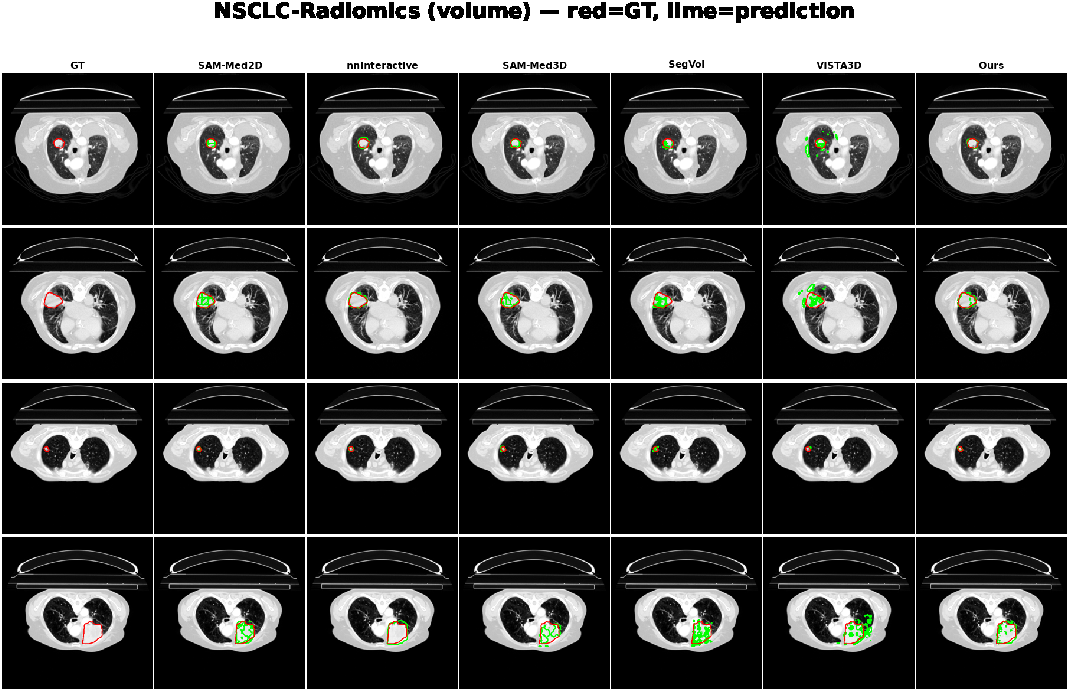
\includegraphics[width=\textwidth]{figures/fig_qual_nsclc_volume.pdf}
  \caption{NSCLC-Radiomics whole-volume overlays for the same four
  patients as in Figure~\ref{fig:qual-cross} (red~=~GT,
  lime~=~prediction; Ours \(60\)-step, \(R{=}1\)). Patch crops in
  Figure~\ref{fig:qual-cross} use the matched \(64^3\) regions from
  these volumes.}
  \label{fig:qual-nsclc-vol}
\end{figure*}

\subsection{Ablation: Steps and Refine Rounds}
Table~\ref{tab:ablation} and Figure~\ref{fig:ablation} vary
inference steps and refine rounds \(R\) on the LIDC positive set
(same checkpoint). Moderate compute (\(40\) steps, \(R{=}2\)) is
sufficient for near-peak Dice; several \(R{=}3\) settings underperform the main \(R{=}2\) operating point,
and \(80\)-step/\(R{=}2\) also does not beat it.
Figure~\ref{fig:qual-ablation} shows the corresponding overlays: coarse
\(30\)-step residuals clean up by \(40\)-step/\(R{=}2\), after which
contours stay visually stable---consistent with the flat Dice curve.

\begin{table}[t]
\centering
\caption{Ablation of inference steps and refine rounds on LIDC
positive test (\(N{=}1658\)).}
\label{tab:ablation}
\begin{tabular}{lcc}
\toprule
Configuration & Dice \(\uparrow\) & IoU \(\uparrow\) \\
\midrule
30-step, \(R{=}3\) & 0.72 & 0.58 \\
40-step, \(R{=}3\) & 0.72 & 0.59 \\
\textbf{40-step, \(R{=}2\)} & \textbf{0.73} & \textbf{0.59} \\
60-step, \(R{=}3\) & 0.72 & 0.58 \\
80-step, \(R{=}2\) & 0.72 & 0.59 \\
\bottomrule
\end{tabular}
\end{table}

\begin{figure}[t]
  \centering
  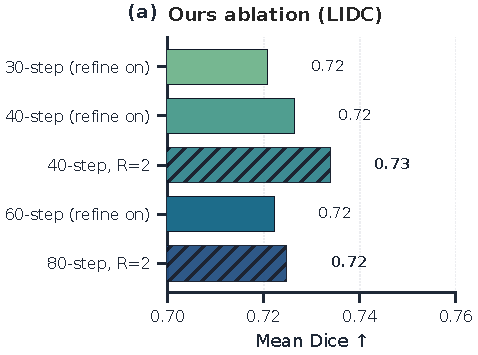
\includegraphics[width=\linewidth]{figures/fig_ablation_steps.pdf}
  \caption{Ablation of RF inference steps and refine rounds on LIDC
  positives. The hatched bar is the main reported config
  (\(40\)-step, \(R{=}2\)).}
  \label{fig:ablation}
\end{figure}

\begin{figure*}[t]
  \centering
  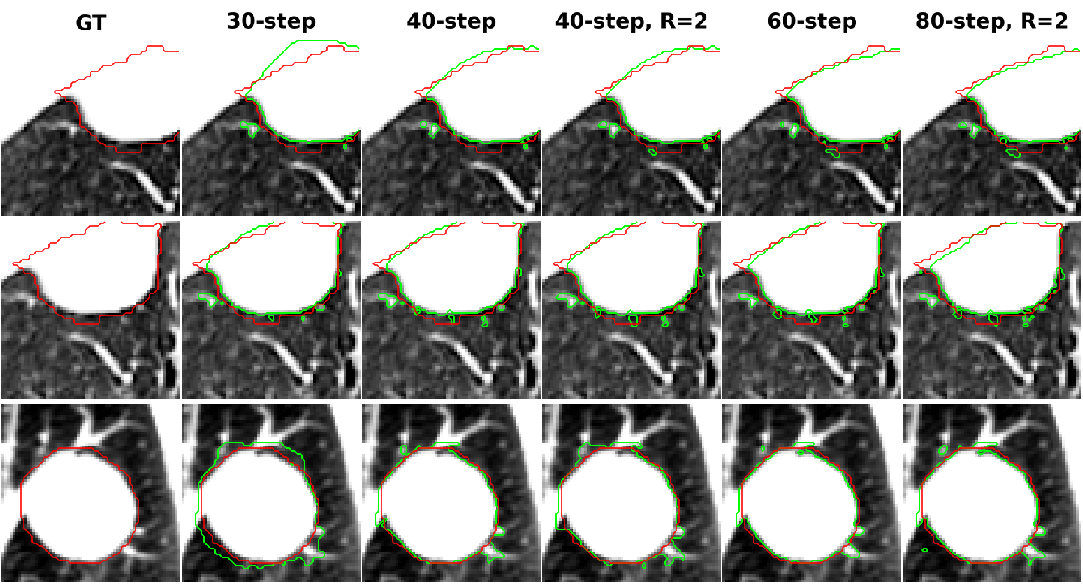
\includegraphics[width=\textwidth]{figures/fig_qual_ablation.pdf}
  \caption{Ablation qualitative overlays on LIDC (red~=~GT,
  lime~=~prediction) for the step/\(R\) settings in
  Table~\ref{tab:ablation}. Contours tighten from \(30\)-step to the
  main \(40\)-step/\(R{=}2\) config and then remain stable.}
  \label{fig:qual-ablation}
\end{figure*}

\subsection{Discussion}
Across Table~\ref{tab:main} and
Figures~\ref{fig:results}--\ref{fig:fp-tradeoff}, the operating point we
report on LIDC (\(40\)-step, \(R{=}2\)) is nearly tied with SAM-Med2D on
true-nodule Dice (Table~\ref{tab:main}) while predicting less spurious mask
volume on the healthy random-box probe
(Table~\ref{tab:healthy_fp}; \(1076\,\mathrm{mm}^3\) vs.\ \(1980\) for
SAM-Med2D and \(4015\) for nnInteractive under the same \(40\)-step/\(R{=}2\)
row). Cross-dataset Dice
(Table~\ref{tab:cross}, Figures~\ref{fig:bench}--\ref{fig:bench-per})
places Ours in a similar competitive tier on MAISI and NSCLC under matched
boxes, without ranking first on every column. The ablation
(Table~\ref{tab:ablation}, Figures~\ref{fig:ablation} and
\ref{fig:qual-ablation}) indicates that additional sampling steps beyond this
point yield little further Dice gain on LIDC. Qualitative overlays
(Figures~\ref{fig:qual-lidc},~\ref{fig:qual-fp},~\ref{fig:qual-cross},
and~\ref{fig:qual-nsclc-vol}) illustrate the same pattern under matched
prompts: competitive recovery on positive cases, sparser predictions on
healthy prompts relative to several object-centric baselines, and transfer
without lesion-mask supervision. These results support the reframing in
Section~\ref{sec:intro}: for region-prompted lung CAD, verifying anomalies
against a healthy generative prior is a useful alternative to interactive
object segmentation when false positives are costly.

% =============================================================
\section{Scope, Limitations, and Conclusion}
\label{sec:conclusion}

\subsection{Scope}
We study \emph{region-prompted} lung CT: a candidate box is already
available, and the system must verify whether that region contains
abnormal tissue and localize it. Within this setting the method does not require lesion-type labels at
training time; any localized finding that deviates from normal parenchyma can
produce a residual (we do not report subtype-stratified Dice).
The framework applies wherever (i)~weak box or slice-wise prompts
exist and (ii)~a corpus of nodule-free lung patches can be curated
to learn the healthy prior. Broader organs and modalities are a
natural extension but require re-training the healthy generative
model on the corresponding normal tissue; they are left to future
work.

\subsection{Limitations}
\begin{itemize}
    \item \textbf{Inference cost.} RePaint-style sampling with
    iterative residual refinement is slower than a single forward
    pass of an interactive foundation model. Rectified-flow
    sampling and fewer refine rounds mitigate latency, but
    distillation or consistency models remain attractive for
    clinical throughput.

    \item \textbf{Candidate dependence.} We assume a region prompt
    (detector, radiologist, or coarse clinical box). The method is
    not a free-search detector; empty or poorly placed boxes can
    still induce residuals from normal anatomical variability.

    \item \textbf{Patch geometry.} The $64^3$ operating resolution
    may clip very large or diffuse findings at patch boundaries;
    whole-volume tiling helps, but multi-scale hierarchical
    inference is future work.

    \item \textbf{Domain of the prior.} The generative model is
    trained on healthy lung CT. Positive evaluations on MAISI and
    NSCLC use the same lung prior; transfer to other organs or
    modalities needs a matching healthy corpus and is left to
    future work.
\end{itemize}

\subsection{Conclusion}
We reframed weakly supervised lung anomaly segmentation---weak in the
sense of box prompts at inference, with no lesion masks at training---as
\emph{region-prompted anomaly verification}: learn a 3D rectified-flow
prior of healthy parenchyma, treat interactive boxes as inpainting holes,
and localize anomalies as residuals against the healthy counterfactual,
sharpened by iterative residual refinement. Under matched prompts, the
approach matches the strongest interactive baseline on LIDC true-nodule
Dice (\(0.73\)), remains in a competitive tier on MAISI and NSCLC, and is
more conservative on healthy random boxes (\(1076\,\mathrm{mm}^3\) mean
predicted volume vs.\ \(1980\) for SAM-Med2D and \(4015\) for
nnInteractive under the reported \(40\)-step/\(R{=}2\) configuration).
These results support generative healthy inpainting as a complementary
alternative to interactive object segmentation when a low false-positive
rate is critical in lung CT CAD.

% =============================================================
\section*{Acknowledgments}
[Omitted for anonymous review.]

% =============================================================
\clearpage
\section*{Supplementary Material}

\subsection*{Default Hyperparameters}
\begin{table}[h]
\centering
\caption{Default hyperparameters used in our method.}
\label{tab:hparams}
\begin{tabular}{@{}ll@{}}
\toprule
\textbf{Setting} & \textbf{Value} \\
\midrule
Patch size & \(64\times 64\times 64\) \\
Spacing & \(0.7\times 0.7\times 1.5\,\mathrm{mm}\) \\
HU window & \([-1000,\,400]\) \\
Scheduler & Rectified flow (continuous) \\
Train timesteps \(T\) & \(1000\) \\
U-Net channels & \([64,128,128,128]\) \\
Objective & \(\ell_1\) velocity regression \\
Learning rate & \(10^{-4}\) \\
Inference steps \(N\) & \(40\) \\
Refine rounds \(R\) & \(2\) \\
Residual threshold \(\tau\) & \(0.05\) \\
Search dilation \(\rho\) & \(2\) \\
Box padding \(p\) & \(2\) voxels \\
Min.\ hole voxels \(\eta\) & \(8\) \\
Morphology & off \\
\bottomrule
\end{tabular}
\end{table}

% =============================================================
\bibliography{AAAI2027_paper}

\end{document}
